\documentclass[titlepage]{article}

\usepackage[letterpaper,margin=1in,footskip=0.25in]{geometry}
\usepackage[hidelinks]{hyperref}
\usepackage{fancyhdr}
\usepackage{csquotes}
\usepackage{amsmath}
\usepackage{amssymb}
\usepackage{tikz}
\usepackage[nottoc,notlof,notlot]{tocbibind}

\MakeOuterQuote{"}

\numberwithin{figure}{section}

\usetikzlibrary{calc,positioning,through}

\newcommand{\R}{\mathbb{R}}
\newcommand{\C}{\mathbb{C}}
\newcommand{\F}{\mathbb{F}}
\newcommand{\dq}[4][]{``#2"#1 \cite[#4]{#3}.}

\newcommand{\Blu}{$\color{blue!30}B$}
\newcommand{\Red}{$\color{red!30}R$}
\newcommand{\Gre}{$\color{green!30}G$}
\newcommand{\Whi}{$W$}

\renewcommand{\labelitemiii}{\scriptsize$\blacksquare$}

\title{GIEP Notes}
\author{Steven Labalme}
\date{\today}

\begin{document}




\pagenumbering{gobble}
\maketitle



\pagenumbering{roman}
\tableofcontents
\listoffigures
\newpage



\pagenumbering{arabic}
\pagestyle{fancy}
\fancyhf{}
\rfoot{Labalme \thepage}
\renewcommand{\headrulewidth}{0pt}
\section{Vector Spaces}
\subsection{$\R^n$ and $\C^n$}
From \cite{bib:Axler}.
\begin{itemize}
    \item Assumed familiarity with the set $\R$ of real numbers.
    \item \textbf{Complex number}: An ordered pair $(a,b)$, where $a,b\in\R$, but we will write this as $a+bi$.
    \begin{itemize}
        \item The set of all complex number is denoted by $\C$:
        \begin{equation*}
            \C = \{a+bi:a,b\in\R\}^[\footnote{The complex numbers equal the set of numbers $a+bi$ such that $a$ and $b$ are elements of the real numbers.}^]
        \end{equation*}
        \item Definitions of \textbf{addition} and \textbf{multiplication} on $\C$ are given, but I know these.
    \end{itemize}
    \item Properties of complex arithmetic:
    \begin{itemize}
        \item \textbf{Commutativity}: $\alpha+\beta=\beta+\alpha$ and $\alpha\beta=\beta\alpha$ for all $\alpha,\beta\in\C$.
        \item \textbf{Associativity}: $(\alpha+\beta)+\lambda=\alpha+(\beta+\lambda)$ and $(\alpha\beta)\lambda=\alpha(\beta\lambda)$ for all $\alpha,\beta,\lambda\in\C$.
        \item \textbf{Identities}: $\lambda+0=\lambda$ and $\lambda 1=\lambda$ for all $\lambda\in\C$.
        \item \textbf{Additive inverse}: For every $\alpha\in\C$, there exists a unique $\beta\in\C$ such that $\alpha+\beta=0$.
        \item \textbf{Multiplicative inverse}: For every $\alpha\in\C$ with $\alpha\neq0$, there exists a unique $\beta\in\C$ such that $\alpha\beta=1$.
        \item \textbf{Distributive property}: $\lambda(\alpha+\beta)=\lambda\alpha+\lambda\beta$ for all $\lambda,\alpha,\beta\in\C$.
    \end{itemize}
    \item \dq{The properties above are proved using the familiar properties of real numbers and the definitions of complex addition and multiplication}{bib:Axler}{3}
    \item $\F$ stands for $\R$ or $\C$.
    \begin{itemize}
        \item Any theorem proved with $\F$ holds when $\F$ is replaced with $\R$ and when $\F$ is replaced with $\C$.
    \end{itemize}
    \item \textbf{Scalar}: A number or magnitude. This word is commonly used to differentiate a quantity from a \textbf{vector} quantity.
    \item Subtraction and division are defined.
    \item Properties of exponents are defined.
    \item The set $\R^2$, which can be conceived as a plane, is the set of all \textbf{ordered pairs} of real numbers:
    \begin{equation*}
        \R^2 = \left\{ (x,y):x,y\in\R \right\}
    \end{equation*}
    \item The set $\R^3$, which can be conceived as ordinary space, is the set of all \textbf{ordered triples} of real numbers:
    \begin{equation*}
        \R^3 = \left\{ (x,y,z):x,y,z\in\R \right\}
    \end{equation*}
    \item \dq
        {Suppose $n$ is a nonnegative integer. A \textbf{list} of \textbf{length} $n$ is an ordered collection of $n$ elements (which might be numbers, other lists, or more abstract entities) separated by commas and surrounded by parentheses. A list of length $n$ looks like this:
        \begin{equation*}
            (x_1,\dots,x_n)
        \end{equation*}
        Two lists are equal if and only if they have the same length and the same elements in the same order}
    {bib:Axler}{5}
    \item \textbf{Ordered pair}: A list of length 2.
    \item \textbf{Ordered triple}: A list of length 3.
    \item \textbf{$n$-tuple}: A list of length $n$.
    \item Although lists are sometimes discussed without specifying their length, a list must, by definition, have a finite length, i.e. $(x_1,x_2,\dots)$ is not a list.
    \item A list of length 0 looks like this: $()$.
    \begin{itemize}
        \item Such an object is defined to avoid trivial exceptions to theorems.
    \end{itemize}
    \item Lists vs. \textbf{sets}: In lists, order matters and repetitions have meaning. In sets, order and repetitions are irrelevant.
    \item \dq
        {$\mathbf{\F^n}$ is the set of all lists of length $n$ of elements of $\F$:
        \begin{equation*}
            \F^n = \left\{ (x_1,\dots,x_n):x_j\in\F\text{ for }j=1,\dots,n)\right\}
        \end{equation*}
        For $(x_1,\dots,x_n)\in\F^n$ and $j\in\left\{ 1,\dots,n \right\}$, we say that $x_j$ is the $j^\text{th}$ \textbf{coordinate} of $(x_1,\dots,x_n)$}
    {bib:Axler}{6}
    \item For help in conceiving higher dimensional spaces, consider reading \emph{Flatland: A Romance of Many Dimensions} by Edwin A. Abbot. This is an amusing account of how $\R^3$ would be perceived by creatures living in $\R^2$.
    \item \textbf{Addition} (in $\F^n$): Add corresponding coordinates:
    \begin{equation*}
        (x_1,\dots,x_n)+(y_1,\dots,y_n)=(x_1+y_1,\dots,x_n+y_n)
    \end{equation*}
    \item For a simpler notation, use a single letter to denote a list of $n$ numbers.
    \begin{itemize}
        \item \textbf{Commutativity} (of addition in $\F^n$): If $x,y\in\F^n$, then $x+y=y+x$.
        \item However, the proof still requires the more formal, cumbersome list notation$^[$\footnote{Note that $\blacksquare$ means "end of the proof."}$^]$.
    \end{itemize}
    \item $\mathbf{0}$: The list of length $n$ whose coordinates are all 0:
    \begin{equation*}
        0=(0,\dots,0)
    \end{equation*}
    \begin{itemize}
        \item Although the ambiguity in the use of "0" on the left vs. right side of the equation may seem confusing, context can always differentiate between which definition is needed.
    \end{itemize}
    \item A picture can help visualize $\R^2$ because $\R^2$ can be sketched on 2-dimensional surfaces such as paper.
    \begin{figure}[h]
        \centering
        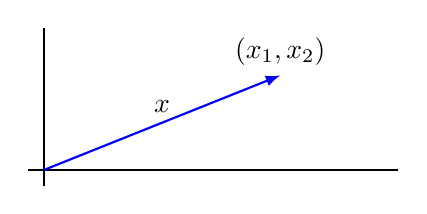
\begin{tikzpicture}[every node/.append style={above,black}]
            \draw (-0.2,0) -- (4.5,0);
            \draw (0,-0.2) -- (0,1.8);
            \draw[blue,thick,-latex] (0,0) -- node{$x$} (3,1.2) node{$(x_1,x_2)$};
        \end{tikzpicture}
        \caption{$x\in\R^2$ can be conceived as a point or a vector.}
        \label{fig:axesvector}
    \end{figure}
    \begin{itemize}
        \item A typical element of $\R^2$ is a point $x=(x_1,x_2)$.
        \item However, points are generally though of as an arrow starting at the origin and ending at $x$, as shown below.
        \item When thought of as an arrow, $x$ is called a \textbf{vector}.
        \item When translated without varying length or direction, it is still the same vector.
        \item Remember that these pictures are aids --- although we cannot visualize higher dimensional vector spaces, the algebraic elements are as rigorously defined as those of $\R^2$.
    \end{itemize}
    \item Addition has a simple geometric interpretation in $\R^2$.
    \item If we want to add $x+y$, slide $y$ so that its initial point coincides with the terminal point of $x$. The sum is the vector from the tail of $x$ to the head of $y$.
    \begin{figure}[h]
        \centering
        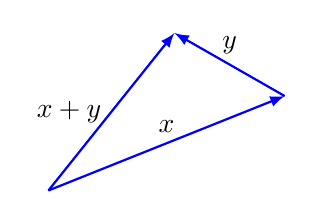
\begin{tikzpicture}[
            every node/.append style={black},
            every path/.append style={blue,thick,-latex}
        ]
            \coordinate (a) at (0,0);
            \coordinate (b) at (3,1.2);
            \coordinate (c) at (1.6,2);

            \draw (a) -- node[above]{$x$}   (b);
            \draw (b) -- node[above]{$y$}   (c);
            \draw (a) -- node[left] {$x+y$} (c);
        \end{tikzpicture}
        \caption{Vector addition.}
        \label{fig:addvectors}
    \end{figure}
    \item \dq
        {For $x\in\F^n$, the \textbf{additive inverse} of $x$, denoted $-x$, is the vector $-x\in\F^n$ such that
        \begin{equation*}
            x+(-x)=0
        \end{equation*}
        In other words, if $x=\left( x_1,\dots,x_n \right)$, then $-x=\left( -x_1,\dots,-x_n \right)$}
    {bib:Axler}{9}
    \begin{figure}[h]
        \centering
        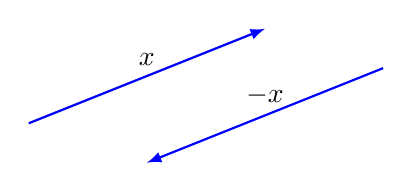
\begin{tikzpicture}[
            every node/.append style={above,black},
            every path/.append style={blue,thick,-latex}
        ]
            \coordinate (a) at (0,0);
            \coordinate (b) at (3,1.2);

            \draw (a) -- node{$x$} (b);
            \draw ($(b)+(1.5,-0.5)$) -- node{$-x$} ($(a)+(1.5,-0.5)$);
        \end{tikzpicture}
        \caption{A vector and its additive inverse.}
        \label{fig:invvectors}
    \end{figure}
    \begin{itemize}
        \item For $x\in\R^2$, $-x$ is the vector parallel to $x$ with the same length but in the opposite direction.
    \end{itemize}
    \item \textbf{Product (scalar multiplication)}: When multiplying $\lambda\in\F$ and $x\in\F^n$, multiply each coordinate of $x$ by $\lambda$:
    \begin{equation*}
        \lambda\left( x_1,\dots,x_n \right)=\left( \lambda x_1,\dots,\lambda x_n \right)
    \end{equation*}
    \begin{figure}[h]
        \centering
        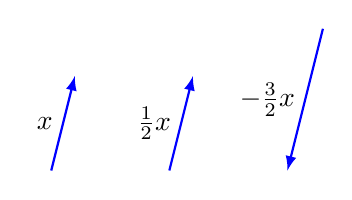
\begin{tikzpicture}[
            every node/.append style={left,black},
            every path/.append style={blue,thick,-latex}
        ]
            \coordinate (a) at (0,0);
            \coordinate (b) at (0.3,1.2);

            \draw (a) -- node{$x$} (b);
            \draw ($(a)+(1.5,0)$) -- node{$\tfrac{1}{2}x$} ($(b)+(1.5,0)$);
            \draw (3.45,1.8) -- node{$-\tfrac{3}{2}x$} ($(a)+(3,0)$);
        \end{tikzpicture}
        \caption{Scalar multiplication.}
        \label{fig:multvector}
    \end{figure}
    \item \textbf{Field}: A \dq[ of complex arithmetic (see earlier in this section)]{set containing at least two distinct elements called 0 and 1, along with operations of addition and multiplication satisfying all the properties}{bib:Axler}{10}
\end{itemize}


\subsection{Definition of Vector Space}
\begin{itemize}
    \item \textbf{Addition (on a set \emph{V})}: \dq{A function that assigns an element $u+v\in V$ to each pair of elements $u,v\in V$}{bib:Axler}{12}
    \item \textbf{Scalar multiplication (on a set \emph{V})}: \dq{A function that assigns an element $\lambda v\in V$ to each $\lambda\in\F$ and each $v\in V$}{bib:Axler}{12}
    \item \textbf{Vector space}: \dq
        {A set $V$ along with an addition and a scalar multiplication on V such that the following properties hold:}
    {bib:Axler}{12}
    \begin{description}
        \item[commutativity] \hfill \\ $u+v=v+u$ for all $u,v\in V$
        \item[associativity] \hfill \\ $(u+v)+w=u+(v+w)$ and $(ab)v=a(bv)$ for all $u,v,w\in V$ and all $a,b\in \F$
        \item[additive identity] \hfill \\ There exists an element $0\in V$ such that $v+0=v$ for all $v\in V$
        \item[additive inverse] \hfill \\ For every $v\in V$, there exists $w\in V$ such that $v+w=0$
        \item[multiplicative identity] \hfill \\ $1v=v$ for all $v\in V$
        \item[distributive properties] \hfill \\ $a(u+v)=au+av$ and $(a+b)v=av+bv$ for all $a,b\in\F$ and all $u,v\in V$
    \end{description}
    \item To be more precise, $V$ depends on $\F$, so sometimes we say $V$ is a \textbf{vector space over $\F$}.
    \begin{itemize}
        \item For example, $\R^n$ is only a vector space over $\R$, not $\C$.
    \end{itemize}
    \item \textbf{Real vector space}: A vector space over $\R$.
    \item \textbf{Complex vector space}: A vector space over $\C$.
    \item $\F^\infty$ is a vector space.
    \item $\F^S$ denotes the set of functions from $S$ to $\F$.
    \begin{itemize}
        \item For example, $\R^{\left[ 0,1 \right]}$ is the \dq{set of real-valued functions on the interval $\left[ 0,1 \right]$}{bib:Axler}{14}
        \item You can think of $\F^n$ as $\F^{\left\{ 1,2,\dots,n\right\}}$.
    \end{itemize}
    \item Elementary properties of vector spaces:
    \begin{itemize}    
        \item A vector space has a unique additive identity.
        \begin{itemize}
            \item Suppose $0$ and $0'$ are both additive identities in V. Then
            \begin{equation*}
                0' = 0'+0 = 0+0' = 0
            \end{equation*}
            The first equality holds due to $0$ being an additive identity. The second holds due to commutativity. The third holds due to $0'$ being an additive identity. Thus, $0=0'$, and $V$ has only one additive identity.
        \end{itemize}
        \item Each element $v\in V$ has a unique additive inverse.
        \begin{itemize}
            \item Same idea:
            \begin{equation*}
                w = w+0 = w+(v+w') = (w+v)+w' = 0+w' = w'
            \end{equation*}
        \end{itemize}
        \item $0v=0\ \forall\ v\in V$, where $0$ on the left side is a scalar and $0$ on the right side is a vector (the additive identity of $V$).
        \begin{itemize}
            \item Since this property asserts something about both scalar multiplication and the additive identity, the distributive property (the only part of the definition of a vector space that connects scalar multiplication and vector addition) must be used in the proof.
            \begin{align*}
                0v &= (0+0)v\\
                0v &= 0v+0v\\
                0v-0v &= 0v+0v-0v\\
                0 &= 0v
            \end{align*}
        \end{itemize}
        \item $a0=0\ \forall\ a\in\F$, where $0$ is a vector.
        \begin{itemize}
            \item Same as above.
        \end{itemize}
        \item $(-1)v=-v\ \forall\ v\in V$, where $-1$ is a scalar and $-v$ is the additive inverse of $v$.
        \begin{equation*}
            v+(-1)v=1v+(-1)v=(1+(-1))v=0v=0
        \end{equation*}
    \end{itemize}
\end{itemize}


\subsection{Subspaces}
\begin{itemize}
    \item \textbf{Subspace}: A subset $U$ of $V$ that is a vector space under the same definition of addition and scalar multiplication as on $V$, e.g., satisfies the following three conditions.
    \begin{description}
        \item[additive identity] \hfill \\ $0\in U$
        \item[closed under addition] \hfill \\ $u,w\in U$ implies $u+w\in U$
        \item[closed under scalar multiplication] \hfill \\ $a\in\F$ and $u\in U$ implies $au\in U$  
    \end{description}
    \item The other conditions can be derived from the above 3.
    \item When we look at subspaces within the differentiable functions, the logical foundation of calculus appears.
    \item The subspaces of $\R^2$ are $\{0\}$, $\R^2$, and any straight line through the origin.
    \item The subspaces of $\R^3$ are $\{0\}$, $\R^3$, any straight line through the origin, and any flat plane through the origin.
    \item \textbf{Sum of subsets}: If $U_1,\dots,U_n$ are subsets of $V$, their \textbf{sum} (denoted $U_1+\cdots+U_n$) is the set of all possible sums of elements of $U_1,\dots,U_n$:
    \begin{equation*}
        U_1+\cdots+U_m = \left\{ u_1+\cdots+u_m:u_1\in U_1,\dots,u_m\in U_m \right\}
    \end{equation*}
    \item The sum of subspaces is the smallest containing subspace.
    \begin{itemize}
        \item Clearly, the sum of subspaces is a subspace (satisfies 3 tenets).
        \item The sum of subspaces contains every original element ($u_1$ plus the $0$ from $u_2$, etc.). Any subspace containing all of these elements must contain every finite sum of them (by definition). Thus, no smaller subspace can be created than that of the sum of every element.
    \end{itemize}
    \item \textbf{Direct sum}: A sum of subspaces where each element of $U_1+\cdots+U_m$ can be written in only one way as a sum $u_1+\cdots+u_m$.
    \begin{itemize}
        \item $U_1\oplus\dots\oplus U_m$ denotes $U_1+\cdots+U_m$ if $U_1+\cdots+U_m$ is a direct sum.
    \end{itemize}
    \item A sum of subspaces is a direct sum if and only if the only way to write $0$ as a sum of elements is by summing the $0$ of each subset.
    \item A sum of subspaces $U$ and $W$ is a direct sum if and only if $U\cap W=\{0\}$.
\end{itemize}
\newpage



\section{Graphs}
From \cite{bib:graph}.
\begin{itemize}
    \item Begins with the K\"{o}nigsberg Bridge Problem and Euler's solution by reducing the land masses to a mathematical \textbf{graph}.
    \item Finding an abstract mathematical model of a concrete problem requires ingenuity and experience. \dq{The primary aim of this chapter is to provide the reader with some of this experience by presenting several real-world problems and showing how they can be formulated in mathematical terms}{bib:graph}{277-78}
    \item Considers the Three Houses--Three Utilities Problem.
    \item Deeply considers Instant Insanity (stack four cubes, each with one of four colors on each face, in such a way that every color is represented on every side of the column):
    \begin{figure}[h!]
        \centering
        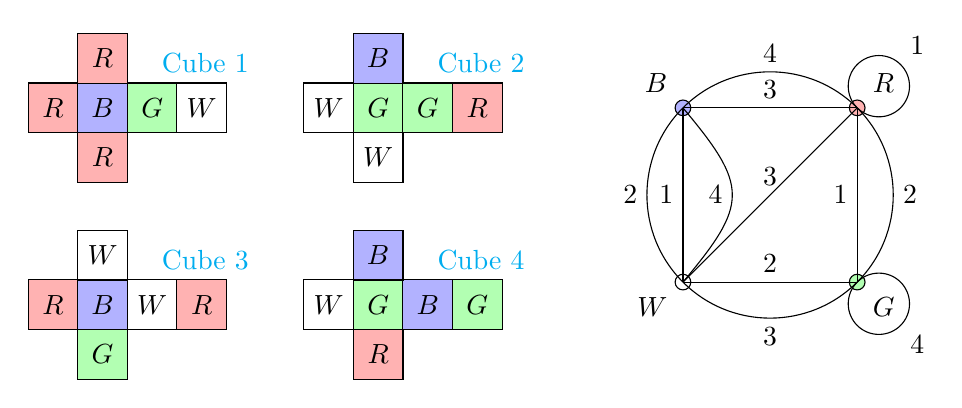
\begin{tikzpicture}
            \colorlet{rex}{red!30}
            \colorlet{blx}{blue!30}
            \colorlet{grx}{green!30}
    
    
            \begin{scope}[
                node distance=-0.42pt,
                every node/.style={draw,minimum size=6.3mm}
            ]
                \node (a1) [fill=rex]             {$R$};
                \node (b1) [right=of a1,fill=blx] {$B$};
                \node (c1) [right=of b1,fill=grx] {$G$};
                \node (d1) [right=of c1]          {$W$};
                \node (e1) [above=of b1,fill=rex] {$R$};
                \node (f1) [below=of b1,fill=rex] {$R$};
            \end{scope}
            \node [above right,cyan] at (c1.90) {Cube 1};
    
            \begin{scope}[
                node distance=-0.42pt,
                every node/.style={draw,minimum size=6.3mm},
                xshift=35mm
            ]
                \node (a2)                        {$W$};
                \node (b2) [right=of a2,fill=grx] {$G$};
                \node (c2) [right=of b2,fill=grx] {$G$};
                \node (d2) [right=of c2,fill=rex] {$R$};
                \node (e2) [above=of b2,fill=blx] {$B$};
                \node (f2) [below=of b2]          {$W$};
            \end{scope}
            \node [above right,cyan] at (c2.90) {Cube 2};
    
            \begin{scope}[
                node distance=-0.42pt,
                every node/.style={draw,minimum size=6.3mm},
                yshift=-25mm
            ]
                \node (a3) [fill=rex]             {$R$};
                \node (b3) [right=of a3,fill=blx] {$B$};
                \node (c3) [right=of b3]          {$W$};
                \node (d3) [right=of c3,fill=rex] {$R$};
                \node (e3) [above=of b3]          {$W$};
                \node (f3) [below=of b3,fill=grx] {$G$};
            \end{scope}
            \node [above right,cyan] at (c3.90) {Cube 3};
    
            \begin{scope}[
                node distance=-0.42pt,
                every node/.style={draw,minimum size=6.3mm},
                xshift=35mm,yshift=-25mm
            ]
                \node (a4)                        {$W$};
                \node (b4) [right=of a4,fill=grx] {$G$};
                \node (c4) [right=of b4,fill=blx] {$B$};
                \node (d4) [right=of c4,fill=grx] {$G$};
                \node (e4) [above=of b4,fill=blx] {$B$};
                \node (f4) [below=of b4,fill=rex] {$R$};
            \end{scope}
            \node [above right,cyan] at (c4.90) {Cube 4};
    
    
            \begin{scope}[
                node distance=2cm,
                every node/.style={circle,draw,inner sep=2pt},
                xshift=8cm
            ]
                \node (B) [fill=blx]            {};
                \node (R) [right=of B,fill=rex] {};
                \node (W) [below=of B]          {};
                \node (G) [right=of W,fill=grx] {};
            \end{scope}
            \node [above left]  at (B.135)  {$B$};
            \node [above right] at (R.45)   {$R$};
            \node [below left]  at (W.-135) {$W$};
            \node [below right] at (G.-45)  {$G$};
            \draw (B.center) --                             node[above]{3} (R.center);
            \draw (B.center) --                             node[left] {1} (W.center);
            \draw (R.center) --                             node[left] {1} (G.center);
            \draw (W.center) --                             node[above]{2} (G.center);
            \draw (B.center) to[bend left=45]               node[above]{4} (R.center);
            \draw (B.center) to[bend right=45]              node[left] {2} (W.center);
            \draw (R.center) to[bend left=45]               node[right]{2} (G.center);
            \draw (W.center) to[bend right=45]              node[below]{3} (G.center);
            \draw (W.center) --                             node[above]{3} (R.center);
            \draw (B.center) to[bend left=40,distance=13mm] node[left] {4} (W.center);
            \node (Rcirc) [draw,circle through={(R.center)}] at ($(R.45)+(0.2,0.2)$)   {};
            \node (Gcirc) [draw,circle through={(G.center)}] at ($(G.-45)+(0.2,-0.2)$) {};
            \node at (Rcirc.45) [above right] {1};
            \node at (Gcirc.-45) [below right] {4};
        \end{tikzpicture}
        \caption{Four colored cubes and a graphical representation.}
        \label{fig:cubesgraph}
    \end{figure}
    \item Each vertex in Figure \ref{fig:cubesgraph} represents one of the colors. Each edge connects a color on one face of a cube to the color on the opposite face (the cube to which this relationship pertains is identified by the number along the edge).
    \begin{itemize}
        \item For example, \Blu\ is connected to \Red\ by a line with $3$ above it because on \textcolor{cyan}{Cube 3}, the blue face and the red face are on opposite sides of the cube.
    \end{itemize}
    \item Let's take a look at a possible stack and see what we can learn from it and its \textbf{subgraph} (see Figure \ref{fig:stack1graph}).
    \begin{figure}[h!]
        \centering
        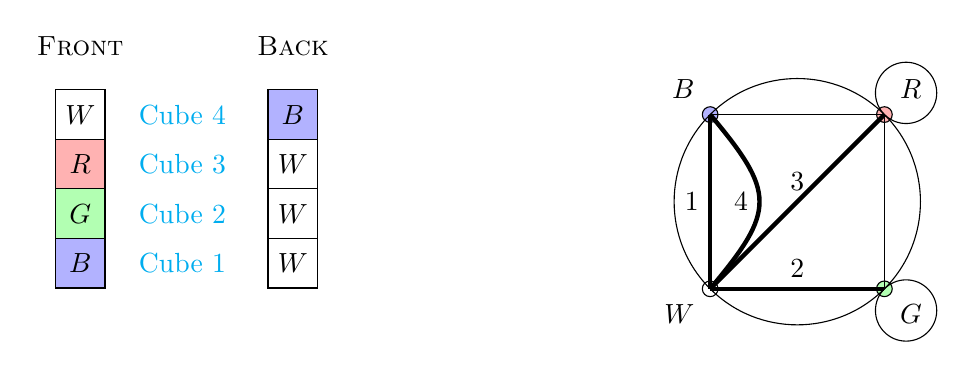
\begin{tikzpicture}[
            node distance=3mm
        ]
            \colorlet{rex}{red!30}
            \colorlet{blx}{blue!30}
            \colorlet{grx}{green!30}
    
    
            \begin{scope}[
                node distance=-0.42pt,
                every node/.style={draw,minimum size=6.3mm}
            ]
                \node (a1)                        {$W$};
                \node (b1) [below=of a1,fill=rex] {$R$};
                \node (c1) [below=of b1,fill=grx] {$G$};
                \node (d1) [below=of c1,fill=blx] {$B$};
            \end{scope}
            \node [above=of a1,font=\scshape] {Front};
            \node [right=of a1,cyan] {Cube 4};
            \node [right=of b1,cyan] {Cube 3};
            \node [right=of c1,cyan] {Cube 2};
            \node [right=of d1,cyan] {Cube 1};
    
            \begin{scope}[
                node distance=-0.42pt,
                every node/.style={draw,minimum size=6.3mm},
                xshift=27mm
            ]
                \node (a2) [fill=blx]    {$B$};
                \node (b2) [below=of a2] {$W$};
                \node (c2) [below=of b2] {$W$};
                \node (d2) [below=of c2] {$W$};
            \end{scope}
            \node [above=of a2,font=\scshape] {Back};
    
    
            \begin{scope}[
                node distance=2cm,
                every node/.style={circle,draw,inner sep=2pt},
                xshift=8cm
            ]
                \node (B) [fill=blx]            {};
                \node (R) [right=of B,fill=rex] {};
                \node (W) [below=of B]          {};
                \node (G) [right=of W,fill=grx] {};
            \end{scope}
            \node [above left]  at (B.135)  {$B$};
            \node [above right] at (R.45)   {$R$};
            \node [below left]  at (W.-135) {$W$};
            \node [below right] at (G.-45)  {$G$};
            \draw               (B.center) --                                            (R.center);
            \draw [ultra thick] (B.center) --                             node[left] {1} (W.center);
            \draw               (R.center) --                                            (G.center);
            \draw [ultra thick] (W.center) --                             node[above]{2} (G.center);
            \draw               (B.center) to[bend left=45]                              (R.center);
            \draw               (B.center) to[bend right=45]                             (W.center);
            \draw               (R.center) to[bend left=45]                              (G.center);
            \draw               (W.center) to[bend right=45]                             (G.center);
            \draw [ultra thick] (W.center) --                             node[above]{3} (R.center);
            \draw [ultra thick] (B.center) to[bend left=40,distance=13mm] node[left] {4} (W.center);
            \node (Rcirc) [draw,circle through={(R.center)}] at ($(R.45)+(0.2,0.2)$)   {};
            \node (Gcirc) [draw,circle through={(G.center)}] at ($(G.-45)+(0.2,-0.2)$) {};
        \end{tikzpicture}
        \caption{A possible stacking and graph.}
        \label{fig:stack1graph}
    \end{figure}
    \item The reason this stack fails to provide a correct column, front and back, is because too many edges touch white and not enough touch red or green.
    \item Also note that this subgraph represents a feasible stack because each cube is represented once (each number appears once in the subgraph).
    \item Therefore, we can conjecture conditions of the subgraph that will lead to a stack that is solved front-to-back, namely:
    \begin{itemize}
        \item The subgraph will contain all four vertices.
        \item The subgraph will consist of four edges, one from each cube.
        \item The subgraph will have exactly two edges meeting at each vertex.
    \end{itemize}
    \item Following these strictures, several graphs can be easily drawn. One such graph is shown in Figure \ref{fig:stack2graph} in correspondence with two columns (this is also the solution to Pause 1).
    \begin{figure}[h!]
        \centering
        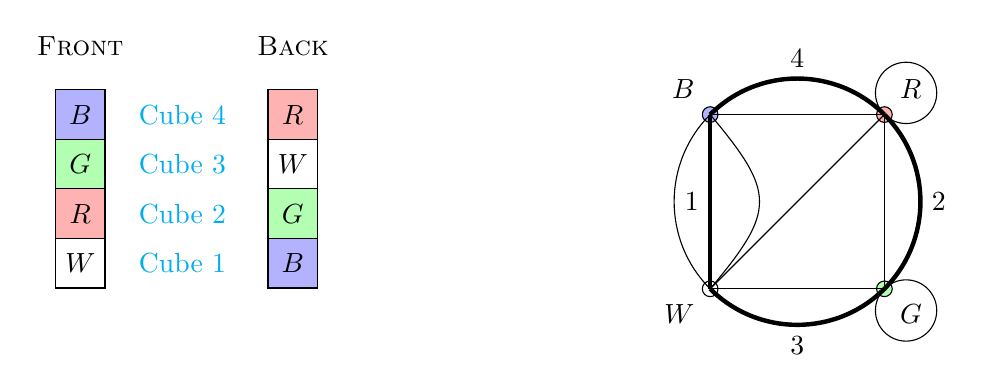
\begin{tikzpicture}[
            node distance=3mm
        ]
            \colorlet{rex}{red!30}
            \colorlet{blx}{blue!30}
            \colorlet{grx}{green!30}
    
    
            \begin{scope}[
                node distance=-0.42pt,
                every node/.style={draw,minimum size=6.3mm}
            ]
                \node (a1) [fill=blx]             {$B$};
                \node (b1) [below=of a1,fill=grx] {$G$};
                \node (c1) [below=of b1,fill=rex] {$R$};
                \node (d1) [below=of c1]          {$W$};
            \end{scope}
            \node [above=of a1,font=\scshape] {Front};
            \node [right=of a1,cyan] {Cube 4};
            \node [right=of b1,cyan] {Cube 3};
            \node [right=of c1,cyan] {Cube 2};
            \node [right=of d1,cyan] {Cube 1};
    
            \begin{scope}[
                node distance=-0.42pt,
                every node/.style={draw,minimum size=6.3mm},
                xshift=27mm
            ]
                \node (a2) [fill=rex]             {$R$};
                \node (b2) [below=of a2]          {$W$};
                \node (c2) [below=of b2,fill=grx] {$G$};
                \node (d2) [below=of c2,fill=blx] {$B$};
            \end{scope}
            \node [above=of a2,font=\scshape] {Back};
    
    
            \begin{scope}[
                node distance=2cm,
                every node/.style={circle,draw,inner sep=2pt},
                xshift=8cm
            ]
                \node (B) [fill=blx]            {};
                \node (R) [right=of B,fill=rex] {};
                \node (W) [below=of B]          {};
                \node (G) [right=of W,fill=grx] {};
            \end{scope}
            \node [above left]  at (B.135)  {$B$};
            \node [above right] at (R.45)   {$R$};
            \node [below left]  at (W.-135) {$W$};
            \node [below right] at (G.-45)  {$G$};
            \draw               (B.center) --                                            (R.center);
            \draw [ultra thick] (B.center) --                             node[left] {1} (W.center);
            \draw               (R.center) --                                            (G.center);
            \draw               (W.center) --                                            (G.center);
            \draw [ultra thick] (B.center) to[bend left=45]               node[above]{4} (R.center);
            \draw               (B.center) to[bend right=45]                             (W.center);
            \draw [ultra thick] (R.center) to[bend left=45]               node[right]{2} (G.center);
            \draw [ultra thick] (W.center) to[bend right=45]              node[below]{3} (G.center);
            \draw               (W.center) --                                            (R.center);
            \draw               (B.center) to[bend left=40,distance=13mm]                (W.center);
            \node (Rcirc) [draw,circle through={(R.center)}] at ($(R.45)+(0.2,0.2)$)   {};
            \node (Gcirc) [draw,circle through={(G.center)}] at ($(G.-45)+(0.2,-0.2)$) {};
        \end{tikzpicture}
        \caption{A front-to-back-solved stacking and graph.}
        \label{fig:stack2graph}
    \end{figure}
    \item Getting the front and back correct is comparably easy to getting the sides correct when playing with the toy.
    \item Graphically, there must be a second subgraph that satisfies the above conditions and is \textbf{edge disjoint} from the first.
    \item \textbf{Edge disjoint} (subgraphs): Two subgraphs that share no edges between them.
    \item Figure \ref{fig:insanesolution} shows two edge disjoint subgraphs superimposed on the same graph.
    \begin{itemize}
        \item These subgraphs correspond to the columns on the left.
        \item Note that the \textcolor{orange!90!black}{orange} subgraph corresponds to the front/back solution while the \textcolor{red!60!blue}{purple} subgraph corresponds to the left/right solution.
    \end{itemize}
    \begin{figure}[h!]
        \centering
        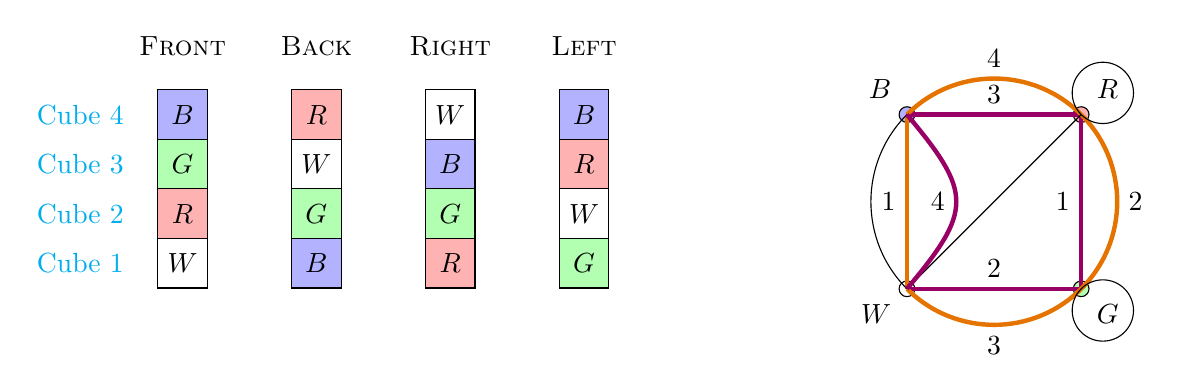
\begin{tikzpicture}[
            node distance=3mm
        ]
            \colorlet{rex}{red!30}
            \colorlet{blx}{blue!30}
            \colorlet{grx}{green!30}
            \colorlet{orx}{orange!90!black}
            \colorlet{pux}{red!60!blue}
    
    
            \begin{scope}[
                node distance=-0.42pt,
                every node/.style={draw,minimum size=6.3mm}
            ]
                \node (a1) at (1.8,0) [fill=blx]             {$B$};
                \node (b1) [below=of a1,fill=grx] {$G$};
                \node (c1) [below=of b1,fill=rex] {$R$};
                \node (d1) [below=of c1]          {$W$};
            \end{scope}
            \node [above=of a1,font=\scshape] {Front};
            \node [left=of a1,cyan] {Cube 4};
            \node [left=of b1,cyan] {Cube 3};
            \node [left=of c1,cyan] {Cube 2};
            \node [left=of d1,cyan] {Cube 1};
    
            \begin{scope}[
                node distance=-0.42pt,
                every node/.style={draw,minimum size=6.3mm},
                xshift=35mm
            ]
                \node (a2) [fill=rex]             {$R$};
                \node (b2) [below=of a2]          {$W$};
                \node (c2) [below=of b2,fill=grx] {$G$};
                \node (d2) [below=of c2,fill=blx] {$B$};
            \end{scope}
            \node [above=of a2,font=\scshape] {Back};
    
            \begin{scope}[
                node distance=-0.42pt,
                every node/.style={draw,minimum size=6.3mm},
                xshift=52mm
            ]
                \node (a3)                        {$W$};
                \node (b3) [below=of a3,fill=blx] {$B$};
                \node (c3) [below=of b3,fill=grx] {$G$};
                \node (d3) [below=of c3,fill=rex] {$R$};
            \end{scope}
            \node [above=of a3,font=\scshape] {Right};
    
            \begin{scope}[
                node distance=-0.42pt,
                every node/.style={draw,minimum size=6.3mm},
                xshift=69mm
            ]
                \node (a4) [fill=blx]             {$B$};
                \node (b4) [below=of a4,fill=rex] {$R$};
                \node (c4) [below=of b4]          {$W$};
                \node (d4) [below=of c4,fill=grx] {$G$};
            \end{scope}
            \node [above=of a4,font=\scshape] {Left};
    
    
            \begin{scope}[
                node distance=2cm,
                every node/.style={circle,draw,inner sep=2pt},
                xshift=11cm
            ]
                \node (B) [fill=blx]            {};
                \node (R) [right=of B,fill=rex] {};
                \node (W) [below=of B]          {};
                \node (G) [right=of W,fill=grx] {};
            \end{scope}
            \node [above left]  at (B.135)  {$B$};
            \node [above right] at (R.45)   {$R$};
            \node [below left]  at (W.-135) {$W$};
            \node [below right] at (G.-45)  {$G$};
            \draw [ultra thick,pux] (B.center) --                             node[above,black]{3} (R.center);
            \draw [ultra thick,orx] (B.center) --                             node[left,black] {1} (W.center);
            \draw [ultra thick,pux] (R.center) --                             node[left,black] {1} (G.center);
            \draw [ultra thick,pux] (W.center) --                             node[above,black]{2} (G.center);
            \draw [ultra thick,orx] (B.center) to[bend left=45]               node[above,black]{4} (R.center);
            \draw                   (B.center) to[bend right=45]                                   (W.center);
            \draw [ultra thick,orx] (R.center) to[bend left=45]               node[right,black]{2} (G.center);
            \draw [ultra thick,orx] (W.center) to[bend right=45]              node[below,black]{3} (G.center);
            \draw                   (W.center) --                                                  (R.center);
            \draw [ultra thick,pux] (B.center) to[bend left=40,distance=13mm] node[left,black] {4} (W.center);
            \node (Rcirc) [draw,circle through={(R.center)}] at ($(R.45)+(0.2,0.2)$)   {};
            \node (Gcirc) [draw,circle through={(G.center)}] at ($(G.-45)+(0.2,-0.2)$) {};
        \end{tikzpicture}
        \caption{A solution to Instant Insanity.}
        \label{fig:insanesolution}
    \end{figure}
\end{itemize}
\newpage



\bibliography{GIEPNotes}
\bibliographystyle{apalike}




\end{document}